\documentclass[a4paper,11pt]{article}

% Padding Requirements
\usepackage[a4paper, margin=1in]{geometry}
% used for double spacing
\usepackage{setspace}
\doublespacing
% Used for images
\usepackage{graphicx}
\usepackage{float}
\graphicspath{{/Users/sloth_mini/Documents/4.1/dissertation/images/}}
% Used for bibliography
\usepackage[style=ieee, sorting=none, backend=biber]{biblatex}
\renewcommand{\bibfont}{\small}
% For math notation
\usepackage{amsmath}
\newcommand{\setA}{\{A\}}
\newcommand{\setB}{\{B\}}
\newcommand{\abrule}{\setA\rightarrow\setB}
% Used for table formatting
\usepackage{booktabs}

\addbibresource{references.bib}

% Do we need a table of contents? I don't think so.
\begin{document}
\title{Deliverable 1: Final Year Dissertation}
\author{
	Sahil Pattni\\ 
	BSc. Computer Science (Honours)\\\\
	Supervisor: Neamat El Gayar
	}
\date{\today}
\maketitle
\pagenumbering{arabic}

\section*{Declaration} 
I, Sahil Manojkumar Pattni, confirm that this work submitted for assessment is my own and is expressed in my own words. Any uses made within it of the works of other authors in any form (e.g., ideas, equations, figures, text, tables, programs) are properly acknowledged at any point of their use. A list of the references employed is included. 
\\
Signed: Sahil Manojkumar Pattni\\
Date: \today
\newpage
\section*{Abstract}
In this digital age, data is being generated at an exponential rate, with data analytics being used by corporations and small businesses alike to produce insights, reduce costs, optimize operations and increase profits.  Generating association rules allows us to find non-intuitive associations that bring new insights to the management, allowing them to leverage this information to maximize their profits. A prime example would be the \textit{'Beers and Diapers'} urban legend, where a company looked at their point-of-sale data and found a strong association between beers and diapers being co-purchased, which seems rather unintuitive.\\
In this study, we will extract a minimum spanning tree (MST) from a data set using machine learning techniques. We will then use this minimum spanning tree to segment products together,  and produce association rules and extract the most interesting ones. The resulting ruleset will be compared to rules generated by the established Apriori Algorithm \cite{apriori}, which is the foundation of association rule mining.  Additionally, we will study how the grouping of the MST compares to clustering algorithms, and how the structure of our MST differs when the dataset is limited to a given city (as opposed to the overall MST), leading to insights that may help the management in such firms make better informed decisions about the type of promotions they would like to run, and the most optimal locations for such.

\newpage
\tableofcontents

\newpage
\section{Introduction}
\subsection{Context}
For businesses which deal with the sale of a heterogeneous physical assets - such as groceries, hypermarkets and select retail outlets - operations such as inventory management and product placement play an instrumental role in determining the business' financial success. These involve asking questions such as:
\begin{itemize}
\item Which products should be placed at the entrance of the store? Which should be placed closer to the exit?
\item Which products will benefit the most by being placed at eye-level?
\item Which products should be placed next to each other to maximize the purchase volume?
\end{itemize}
One way to find optimal solutions for such questions is to employ the use of Association Rule Mining (also known as Market Basket Analysis). This set of techniques assess frequent itemsets (e.g. from sales data) and generate association rules between products. Several algorithms and techniques exist for association rule mining, such as the Apriori Algorithm and FP-Growth \cite{fp_growth}. One problem with these algorithms is that they tend to generate an enormous amount of rules, of which many of the rules themselves are large This makes it grossly inconvenient for the end-user to retrieve any actionable information from the results.\\
What we will do is construct a network of products - where each vertice represents a product or product category, and an edge between two vertices represents the simultaneous occurrence of the the two products. The result is a graph (i.e. a network), whose architecture is visually informative of the products and their associations.  The insights that can be gained from the MST can help the management of the mentioned businesses to maximize their profit.

\subsection{Aims}
The aim of this study is to study the effectiveness of a minimum spanning tree as a market basket analysis tool - from product clustering to association rule mining.  Additionally, we will determine how the architecture of the MST will change during and after large events such as promotions. The model will be tested on a relatively large dataset of sales data.

\subsection{Objectives}
The research objectives for this project have been laid out below, in the order that they will be carried out.
\begin{enumerate}
\item Acquire a suitable dataset upon which the MST can be constructed.

\item \label{optimal} Explore and evaluate MST extraction algorithms.
\\(While Prim's \cite{prims}\cite{prims_og} and Kruskal's \cite{kruskal} algorithms are the most commonly used methods to extract the MST from a graph, research has been conducted on more efficient ways to extract the MST using machine learning techniques such as K-Means, and these will be discussed in the literature review (see Section \ref{related-work}).

\item Generate an undirected graph $G(E,V)$ where the edges $E$ are the correlation values between the product vertices.

\item Extract a minimum spanning tree from this graph using the technique determined in step \ref{optimal}. 

\item Analyze this MST and use its architecture to determine product clusters and generate association rules.

\item Generate association rules using the Apriori and FP-Growth algorithm and compare them in both their time complexity and their \textit{'interestingness'} (i.e. the unintuitive rules they generate).

\item Validate the product grouping present in the MST against parent categories (if present), and a clustering algorithm (e.g.  such as the K-Means algorithm).
\end{enumerate}

\newpage
\section{Background}
\subsection{Core Concepts} % TODO: Maybe change title?
\subsubsection{Graphs}
\begin{figure}[H]
\centering
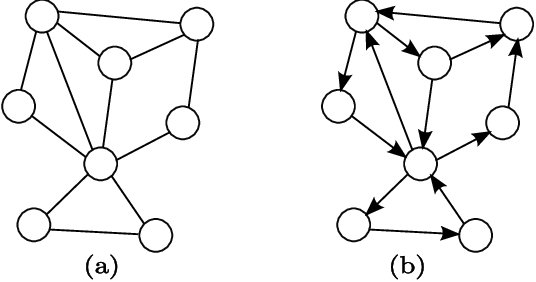
\includegraphics[scale=1.5]{graph-example}
\caption{Undirected and Directed Graphs}
\label{fig:graph.example}
\end{figure}
In discrete mathematics and more specifically - graph theory, a graph is a data structure that contains a set of nodes (i.e. vertices) connected by lines (i.e. edges).  These edges may be directed - such as in Figure \ref{fig:graph.example}:(a), or undirected - such as in Figure \ref{fig:graph.example}:(b). A graph $G$ with a set of vertices $V$ and a set of edges $E$ can be represented via the notation $G = (V,E)$. For the purposes of our research, we will be focusing on undirected graphs, where the weight between two vertices is the same in both directions.
\subsubsection{Minimum Spanning Trees}
Given an undirected $G = (V,E)$,  a \textit{spanning tree} can be described as a subgraph that is a tree which includes all the vertices $V$ of $G$ with the minimum number of edges required. A \textit{minimum spanning tree} (MST) is the spanning tree with the smallest sum of edge weights.  This means that if the graph has $n$ vertices, each spanning tree - including the minimum spanning tree - will have $n-1$ edges.
\subsection{Binary Purchase Vectors}
Binary purchase vectors play an instrumental role in the construction of the MST, helping us determine the association between products. What is a binary purchase vector, however? It is a vector whose length is the number of unique products in the dataset, where each element is a 1 or 0 depending on whether the product was purchasd or not. Imagine a grocer who only sells five items: milk, eggs, bread, apples and oranges. If a customer purchases bread and oranges, the binary purchase vector for that transaction would look like this:
\begin{table}[H]
\centering
\begin{tabular}{@{}ccccc@{}}
\toprule
milk & eggs & bread & apples & oranges \\ \midrule
0    & 0    & 1     & 0      & 1       \\ \bottomrule
\end{tabular}
\end{table}
\subsubsection{Market Basket Analysis and Apriori Rule}
\label{mba_define}
Market Basket Analysis (MBA), also known as Affinity Analysis, is a data mining and analysis technique that identifies co-occurrence patterns between products purchased together, and produces association rules for these products as such: $\abrule$ which implies a strong relationship between the purchase of product $A$ and product $B$. In the case of our \textit{beers and pampers} example, the association rule could be represented as $\{Beers\} \rightarrow \{Pampers\}$. The contents of a purchase basket (i.e. the contents of a customer's basket when they check out) is called a \textit{itemset}, which - as the name suggests - is a set of all the items in the basket.  For example, if a customer had bought detergent, bread and soda, the itemset would be $\{\textit{bread, detergent, soda}\}$. Association rules are generated by looking at different combinations of the itemset (e.g. $\{\textit{bread, soda}\}\rightarrow\{\textit{detergent}\}$ and $\{\textit{soda}\}\rightarrow\{\textit{bread}\}$). 
The equation \cite{num_rules} to calculate the number of rules for an itemset of length $d$ is as follows :\\
\begin{equation}
\textit{number of rules} = \sum\limits_{k=1}^{d-1} \left(\binom{d}{k} \times \sum\limits_{j=1}^{d-k}\binom{d-k}{j}  \right)
\label{eq:numrules}
\end{equation}
Analyzing the equation, it becomes apparent that the problem with association rule generation from itemsets is that the number of rules produced grows exponentially with the size of the itemset, as we can see in Figure \ref{fig:numrules}, using Equation \ref{eq:numrules}.  
\begin{figure}[H]
\centering
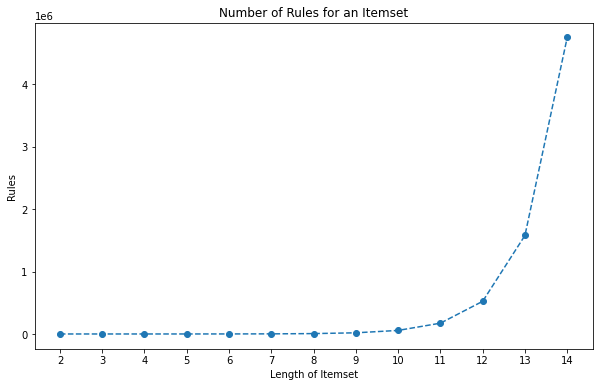
\includegraphics[scale=0.6]{numrules}
\caption{Number of Association Rules for an Itemset}
\label{fig:numrules}
\end{figure}
Clearly, checking all itemsets in a database would be computationally expensive, and so we only look at \textit{frequent itemsets} - itemsets that have a support value above a minimum threshold $\textit{min}_{\textit{support}}$. Even so, checking each itemset's support score via brute force is unacceptably time consuming, therefore we can optimize the search for frequent itemsets using the Apriori Principle \cite{mine}, which states that \textit{all subsets of a frequent itemset must be frequent}. To understand how the Apriori Principle can be applied here, we first look at three key metrics:
\\\textbf{Support}\\
The support of a set of products is the fraction of transactions in which these set of products are present. For example,  for a list of transactions $T$, for the product $X$ where $T(X)$ denotes that the set of transactions in which X was present:
\[
\textit{support}(\{A\}) = \frac{T(A)}{T}
\]
and similarly, 
\[
\textit{support}(\abrule) = \frac{T(A,B)}{T}
\]
denotes the support for the rule $\abrule$. We can prune rules with a low support as they indicate a rule does not occur enough to draw any reasonable conclusions from.
\\\textbf{Confidence}\\
Confidence is the measure of how likely a product will be in a basket given that another product is in it. That is to say,  the confidence of a rule $\abrule$ is the conditional probability that $\setB$ occurs in the basket given that $\setA$ is present. The confidence of a rule can be denoted as:
\[
\textit{confidence}(\abrule) = \frac{T(A, B)}{T(A)} \equiv \frac{\textit{support}(\abrule)}{\textit{support}(\setA)}
\]
\\\textbf{Lift}\\
The lift of a rule $\abrule$ is the rise (i.e. \textbf{lift}) that $\setA$ gives to our $\textit{confidence}(\abrule)$.
\[
\textit{lift}(\abrule) = \frac{confidence(\abrule)}{support(\setB)}
\]
To make this easier to understand, imagine that $\textit{confidence}(\abrule)=0.5$, and $\textit{support}(\setB)=0.4.$ This means that the presence of $\setA$ increases the probability of $\setB$ being in the same basket by $25\%$ ($\frac{0.5}{0.4}=1.25$), therefore providing us with a lift value of 1.25.  A lift value below 1 would indicate that the occurrence of $\setA$ in a basket decreases the likelihood of $\setB$ occurring in the same basket (i.e. a low product association).
\\
As we established above,  the Apriori Principle states that all subsets of a frequent itemset must be frequent.  The Apriori Principle is a result of the \textit{anti-monotone property of support} \cite{anti_monotone}, which means for $\{A,B,C\}$, $\textit{support}(\{A,B\}) \geq \textit{support}(\{A,B,C\})$.  We can use this to prune the frequent itemsets much more efficiently, because if $support(\{A,B\}) < \textit{min}_{\textit{support}}$, then any itemset containing the set $\{A,B\}$ will also fall below $\textit{min}_{\textit{support}}$. Once the frequent itemsets have been pruned,  association rules can be generated from the remaining itemsets.  The resulting association rules can be even further pruned by removing those that fall below a confidence threshold $\textit{min}_{\textit{confidence}}$.  Finally, the remaining rules can be ranked according to their  lift to find the rules with the highest associations.  Figure \ref{fig:prune} is an illustration of how pruning one set $\{A, B\}$ leads to the pruning of all its children.

\begin{figure}[H]\centering
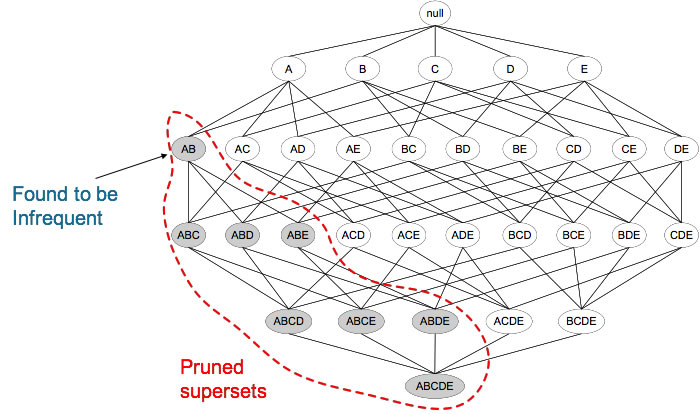
\includegraphics[scale=0.5]{apriori-prune}
\caption{Pruning Infrequent Rules}
\label{fig:prune}
\end{figure}

\subsection{Related Work}
\label{related-work}
\subsubsection{Papers on Association Rules}
\textbf{R. Aggarwal et al.} \cite{mine} proposed a novel algorithm to generate all statistically significant association rules between items in a database, laying the foundations for association rule mining.  Given a set of items $I = I_1, I_2, I_3,...I_m$, the authors define an association rule to be of the form $X \rightarrow I_j$ where X is a set of items such that $X \in I, I_j \notin X$.  The hypothetical database stated was a list of transactions, $T$, where each transaction $t$ was a binary vector of length $m$, representing a basket purchase, where $t[k] = 1$ if $I_k$ been purchased in that basket.  The authors stated that their methodology for association rule mining could be split into two steps: the generation of candidate itemsets, and the generation of statistically significant association rules from these itemsets. \\
To address the first subproblem, the authors provided the pseudo-code for their candidate itemset generation,  where all itemsets possible were generated from tuples (samples) from the database,  and those itemsets whose support score\footnote{see: Section \ref{mba_define}} is above the minimum support threshold are considered candidates (called \textit{large itemsets}).  Since a brute-force check would be sub-optimal  (the authors note this could take up to $2^m$ passes of the database),  the authors devised a methodology to check for candidate itemsets where on the $k^{th}$ pass of the database, they would only check itemsets of length $k$, to see if they satisfied the support constraint. On the $(k+1)^{th}$ pass, they need only check those itemsets that are 1-extensions (i.e.  itemsets extended by exactly one item) of the \textit{large itemsets} found in the previous pass. This is because of what would later be known as the \textit{Apriori Principle}, where if an itemset $Y$ is \textit{large}, then all subsets of $Y$ must also be \textit{large}. Therefore, if they found the itemset $\{A,B\}$ was \textit{small} (i.e. did not satisfy the support constraint), then sets containing $\{A,B\}$ (e.g. $\{A,B, C\}, \{A,B, D\}, \{A,B, C, D\}$) would also be small, and need not be checked. This means, however, that if an itemset $I$ is \textit{large}, then another pass over the dataset would be required to check the support of the subsets of $I$. To avoid this, the authors devised a measure to calculate the expected support, $\bar{s}$, of an itemset,  and use this to measure the support of itemsets $I = (X + I_j)$ not only where $I$ is expected to be large, but also where $X+I_j$ is expected to be small but $X$ is expected to be large, further helping them prune the number of itemsets to check.  The authors proceed to define a method that allows the algorithm to be more memory efficient\footnote{This may no longer be required due to the advances in computational power in the the 27 years since this paper was written.}. The authors also defined method to further prune itemsets from the search, namely \textit{remaining tuples optimization} and \textit{pruning function optimization}.\\
To address the second subprobem,  the authors proposed the following methodology: for each large itemset $Y = I_1, I_2,...I_k, k\geq 2$ from the set of non-pruned large itemsets, generate a set of association rules of form $X \rightarrow I_j$ such that the consequent is $I_j$ and the antecedent (i.e. the precedent set in the rule) is a subset $X$ of $Y$ such that $X$ is of length $k-1$ and $I_j \notin X$. Therefore, each large itemset will produce $k$ rules. From the generated rules, the authors discarded those rules whose confidence scores\footnote{see: Section \ref{mba_define}} fell below the minimum confidence threshold $c$.\\
The authors tested their methodology on a sales dataset with $46,783$ transactions,  with $63$ \textit{items} (in this case, the department from which the customer bought an item). They used a configuration of a minimum support threshold of $1\%$ and a minimum confidence threshold of $50\%$. The rules produced seemed to follow with general intuition, such as:\\
$\{\text{Auto Accessories, Tires}\} \rightarrow \{\text{Automotive Services}\} $\\
Furthermore, the authors assessed the accuracy of their expectation method, by measuring the ratio of correctly estimated itemsets for both small and large, against various values for the minimum support threshold, and visualizing the result. To isolate the effect of their expectation method, they disabled their pruning optimization functions. They were able to conclude that their estimation accuracy was satisfactory, as their accuracy was above 98\% for support thresholds except the first, where it was 96\%.  The authors also tested the effectiveness of their pruning optimization functions, namely the \textit{remaining tuples} and the \textit{pruning function} optimization functions, against multiple minimum support threshold values. They were able to conclude that their pruning efficiency increased as the support threshold increased.
\\\textbf{Critical Analysis}\\
(To be completed)

\subsubsection{Papers on MBA using Trees and Networks}
\textbf{M. Zekić-Sušac et al.} \cite{market_ass} proposed a novel measure for the \textit{interestingness} of association rules,  identifying that a dominant, universally used measure did not exist. The authors' goal was to combine objective measures such as the support, confidence and lift scores with more subjective measures. Instead of the Apriori approach, their methodology has them generate association rules via the \textit{tree-building technique} - which compresses a large database into a Frequent-Pattern tree, citing that this technique was more efficient than the Apriori algorithm. The author's employed the heuristical unexpectedness measure(i.e.  significantly contradicting a user's prior beliefs) and the heuristical actionability measure (i.e. if the end user can use the information to their advantage(e.g. a promotion)) as their subjective measures, and a minimum confidence threshold of 51\% as their subjective measure.  Since a subjective measure would require a human subject, the authors' used the estimations of a sales manager from a Croatian retail chain, and stored his responses in binary format for the subjective measures (i.e. 0 if a rule was unexpected else 1, 0 if a rule is not useful else 1). The dataset used for this paper was a real transactional dataset with 14,012 transactions and a set of 1,230 unique items (which was later pruned to 7,006 transactions and a set of 278 products) from the same Croatian retail chain their test subject worked at. The authors then generated association rules from the first-level hierarchical grouping of items from the dataset (items with a minimum support of 25\%),  of which 36 rules were identified as statistically significant.  From this set of rules, only two rules satisfied both subjective measures and the confidence constraint, and therefore these two rules were identified as highly interesting.  The authors then generated association rules from the second-level hierarchical grouping of items, where items that represented the same product (but had different a manufacturer, brand etc.) were grouped together. Of the rules generated, 15 satisfied their confidence constraints and had a support value able 10\%. 5 rules from this set satisfied both their subjective and objective measures,  more than the previous experiment  The authors were able to conclude that the increase in accuracy that resulted from the second level of grouping which generalized the products.\\
\textbf{Critical Analysis}\\
(To be completed)
\\\\
% MAIN MST PAPER
\textbf{M. A. Valle et al.} \cite{mst_paper} proposed a novel methodology to study the structure and behavior of consumer market baskets from the topology of a minimum spanning tree which represented the interdependencies between products, and use this information to complement the association rule generation process. The input to their proposed methodology was a correlation matrix between the set of all one-hot encoded purchase vectors such that each vector denoted the presence or non-presence of each product from the dataset in that vector.  The dataset used for the MST construction was a list of $1,046,804$ transactions containing a set of $3,240$ unique products from a large supermarket chain branch in Santiago, Chile.  When building this correlation matrix, the authors opted to use the Pearson's Coefficient (which is equivalent to the coefficient $\phi$ for binary data such as theirs) over the traditionally used Jaccard distance to compute the similarity between the binary product vectors, as the former provides both a positive and negative association between products. Additionally,  they used the distance function $d_{ij} = \sqrt{2(1-\phi_{ij}}$ to transform the correlation matrix into a distance measurement (i.e. the weight of the edges).  The authors constructed a MST for 220 product subcategories, and noted that there was a significant level of grouping between product sub-categories that belonged to the same parent category.  To remove edges from the MST that were not statistically significant,  the authors used the mutual information \cite{measure} measure $\sum\limits_{x,y}log_2 \frac{r(x,y)}{p(x)q(y)}$ between product subcategories $p$ and $q$, and were able to prune 14 edges, all of which were connected to a terminal node, therefore effectively pruning 14 vertices from the MST too. To identify the most influential regions of the MST, the authors defined an influence zone of distances that were in the $10^{th}$ percentile. To generate meaningful association rules,  for each MST product $i$, the authors ran a search for the set of all association rules $R_i$ such that $P_i \rightarrow P_j (i \neq q)$. Then from the resulting set of rules, they searched for rules that obeyed $P_i \rightarrow P_m$ where $m$ a product node connected to the product $i$ in the minimum spanning tree.  For both resulting sets of rules for each product, the mean of their lift scores were observed, and the authors determined that the rules that were reinforced by the MST had a higher mean, and that a majority of these rules had a lift score above the $90^{th}$ percentile. 
\\
To identify the clusters each of the products should be identified under, the authors constructed a hierarchical tree using the average linkage clustering method, and by using an unspecified cut distance, they were able to produce 17 taxonomic groups (i.e. clusters). Cross-referencing their results with the actual parent categories of the products, they were able to conclude that the MST did indeed categorize the product sub-categories into clusters with a reasonable degree of accuracy. The authors then compared their MST to another methodology, namely the structured association map (SAM) \cite{kim}, using the Jaccard distance as a measure of similarity,  and were able to generate interesting 2x2 rules (i.e. $\{A,B\}\rightarrow\{C, D\}$), all with lift scores above 1.0, with one rule even having a lift score of 106.46. They concluded that while both approaches provided different information, they both visually identify the strongest relationships between the products, and provide useful information to reduce the search space for association rules.
\\\textbf{Critical Analysis}\\
The authors' approach seems to be novel,  thorough and well structured.  Their methodology successfully employed the use of minimum spanning trees to complement the association rule generation process with sound results.  One caveat of their approach is that they only used the MST to generate 1x1 rules (i.e. $\abrule$). Using the distance score in conjunction with the importance function they defined (i.e. $\sum\limits_{k \in K_u}^{} \frac{1}{w_{uk}}$), they could have defined a system to produce $p \times q$ rules (where $ p \geq 1, q \geq 1$;i.e. rules that have one \textit{or more} items in the antecedent and consequent), then rank them using their respective lifts.  Additionally, while the authors did cross reference their clustering results against the real parent categories of the products, they did not compare their results to that of a clustering algorithm (e.g. K-Means), which would have given a reasonable benchmark to compare the results of the MST clustering to. While 1x1 rules are easily understandable and tend to have high lift values when extracted from the MST, $p \times q$ rules would provide a layer of insight as to how a range of products (perhaps a cluster) related to another.

\newpage
\section{Requirements \& Research}
\subsection{Requirements Analysis}
This section will identify both the functional and non-functional requirements required for the implementation of the model proposed in this document. By stating the specific requirements of the model,  it serves as a high-level view of how the model should function. 
 
 % FUNCTIONAL
\begin{table}[H]
\centering
\caption{Functional Requirements}
\begin{tabular}{@{}rll@{}}
\toprule
\textbf{ID} & \textbf{Category} & \textbf{Description}                   \\ \midrule
FR1        & Dataset           & The dataset must not have any empty values. \\
FR2        & Dataset           & The dataset must have a unique identifier for each transaction.\\ 
FR3     &  Model       & A list of binary purchase vectors must be extracted from the dataset.\\
FR4     &  Model       & The model must return a storable data type representation of a MST.\\
FR5    & Model        & The model must produce  $p \times q$ association rules.\\
\bottomrule
\end{tabular}
\label{tab:fr}
\end{table}

% NON-FUNCTIONAL
\begin{table}[H]
\centering
\caption{Non-Functional Requirements}
\begin{tabular}{@{}rll@{}}
\toprule
\textbf{ID} & \textbf{Category} & \textbf{Description}                   \\ \midrule
NFR1       & Dataset         & The dataset must contain at least 500,000 unique transactions.\\
NFR2     & Hardware    & The data inputs and the MST construction will run on a computer\\&&with at least 8 GB of ram, and a quad-core CPU with clock speed\\&&aabove 2.5GHz.\\
\bottomrule
\end{tabular}
\label{nfr}
\end{table}

\subsection{Research Methodology}
\subsubsection{Technical Choices}
We will be building our model on Python 3.8. It is a versatile, fast language with both object-oriented and functional paradigms, with vast support and numerous libraries for data analytics and machine learning, many of which act as an interface for functions written in faster languages such as C/C++. We will be using the following libraries to help optimize our development process:
\begin{itemize}
\item pandas
\item numpy
\item scikit-learn
\item matplotlib
\item graphviz
\item efficient-apriori
\end{itemize}
\subsubsection{Implementation}
The primary objective of this dissertation is to analyze the viability of a framework based on the minimum spanning tree as a 'one-in-all' tool for market basket analysis,  from association rule generation to clustering.  This section will describe how we plan to achieve these goals:\\
A candidate dataset has been identified: a dataset of $~27,000,000$ transactions occurring across multiple branches of a Brazilian gas station store \cite{data_source}. Each row in the dataset contains the purchase information for a particular product for a given transaction. The dataset has been checked for errors and inconsistencies, and any found have been remedied. Additionally, since the transaction id is an unreliable identifier for a market basket\footnote{transaction numbers reset once they have reached an upper limit, transaction ids are not synced across stores so the same transaction id could refer to multiple transactions across different stores.}, we have assigned each row a unique alphanumeric code consisting of the purchase's transaction number, city and date, which will act as a robust unique identifier for each basket. F Additionally, we have removed redundant or unnecessary features from the dataset, this will allow us to make quicker passes through all the data when generating the binary purchase vectors.  Once the dataset is prepared, we will need to extract a binary purchase matrix from the dataset.  Since each product purchase has an assigned transaction number, to find all product purchases in a transaction, we will need one pass of the database. Therefore, to build $n$ binary purchase vectors, we will need $n$ passes of the database (i.e.  a complexity of $O(n)$). This will prove to be quite computationally expensive,  as there are approximately $5,200,000$ unique baskets in our dataset.  Even when only considering $473,641$ baskets with $40$ unique products, the resulting matrix (see Fig. \ref{fig:corrmat}) took over 6 hours to construct.  We will be looking into more efficient ways to generate out input data. \\
\begin{figure}[H]
\centering
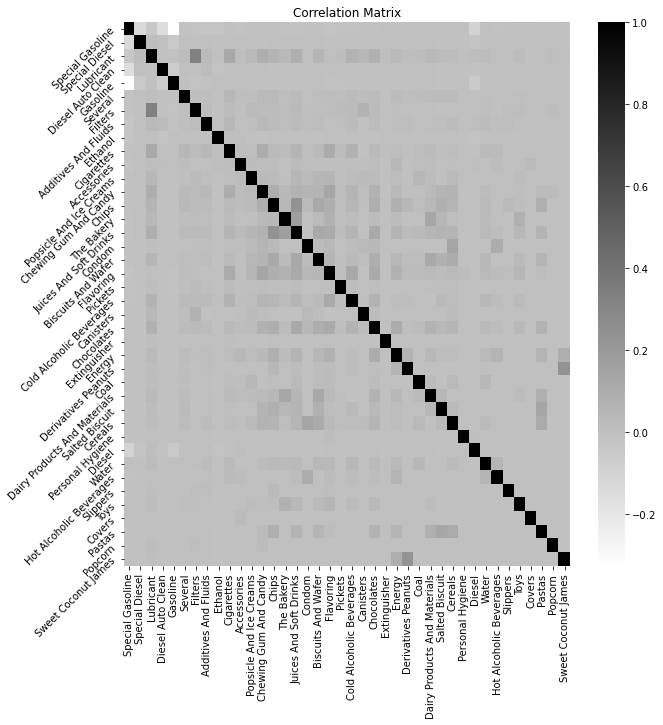
\includegraphics[scale=0.5]{corrmat}
\caption{Correlation Matrix for 473,641 baskets}
\label{fig:corrmat}
\end{figure}
Once the correlation matrix has been generated and a distance function applied, a graph will have to be constructed.  Given the size of our dataset, extracting a MST from our graph using traditional algorithms such as Prim's and Kruskal's may be ineffective, and we may have to look into more recent approaches. For example,  \textbf{C. Zhong et al.} \cite{kmeans_mst} proposed a divide-and-conquer algorithm for extracting a minimum spanning tree based on the K-Means clustering algorithm, which may be worth considering over Prim's and Kruskal's.  Using the appropriate extraction method, we will retrieve our MST from the graph. We will then repeat the above methodology, but after aggregating the products (e.g.  renaming all the brands of lubricant to 'lubricant', similar to the second-level hierarchical grouping in \cite{market_ass}) ,  which will allow us to study how these generalized products affect the structure of the MST. From the resulting minimum spanning trees,  we will then be able to extract the most interesting association rules (i.e. those with the highest statistical significance).  We will also repeat this process several times,  limiting the dataset to a particular city each iteration to observe how the architecture of the MST differs by city as compared to the dataset as a whole.

\newpage
\section{Evaluation Strategy}
Our model will need to evaluated to ensure that:
\begin{enumerate}
\item The model satisfies all the listed functional requirements listed in Table \ref{tab:fr}.
\item We are able to extract high-value association rules from the MST.
\item The MST architecture indicates a level of product grouping that is consistent with their parent subcategories.
\end{enumerate}

\subsubsection*{Functional Requirement Validation}
\texttt{FR1: The dataset must not have any empty values.}\\
To evaluate this, we can pass through the dataset, checking for empty/null values. The result of this evaluation is binary - no empty values found or more than 0 found.\\\\
\texttt{FR2: The dataset must have a unique identifier for each transaction.}\\
To evaluate this, we can a script to validate if each product purchase's associated transaction identifier matches the expected value. The result of this evaluation is also binary - either all unique transaction identifiers are as expected, or otherwise.\\\\
\texttt{FR3: A list of binary purchase vectors must be extracted from the dataset.}\\
Using the unique transaction identifier for each product in the database, we can generate our binary purchase vectors.  To evaluate this, we can ascertain if the dimensions matrix of binary purchase vectors are consistent with our expected value.

\subsubsection*{Rule "Interestingness" Validation}
There are two ways to validate the \textit{interestingness} of an association rule:
\begin{itemize}
\item Objective measures: Metrics such as the support, confidence and lift scores will be used to rank the rule and evaluate its relative position against all the other rules.  Additionally, we will be generating a greater number of association rule using the Apriori algorithm,  and observing tour rule's relative position to these rules ranked by the aforementioned metrics.
\item Subjective measures: Due to the ongoing pandemic, we will not be pursuing subjective measures to validate our rules, as subjective evaluation will require a third party to be present.
\end{itemize}

\subsubsection*{MST Grouping Validation}
One way to validate the MST is to check the grouping of products in the MST. Ideally,  grouping of similar products should be present (e.g. strong grouping between dairy products). We can set a threshold on the edge distance, such that any products within that threshold radius can be considered a cluster.  One objective way to evaluate this cluster is to build a confusion matrix with the products against their parent categories and evaluate the proportion of products grouped together under their correct parent category. It would also be interesting to compare the results of the MST grouping to the clusters generated by an unsupervised clustering algorithm such as the K-Means clustering algorithm.
%%
%%\newpage
%%\section{Evaluation Strategy}
%%
%%\newpage
%\section{Project Management}


% Keep references on new page
\newpage
\printbibliography

\end{document}